\documentclass[a4paper]{article}

%% Language and font encodings
\usepackage[english, brazil]{babel}
\usepackage[utf8x]{inputenc}
\usepackage[T1]{fontenc}
\usepackage{ifthen}
\usepackage{lipsum}
\usepackage{float}
%% Sets page size and margins
\usepackage[a4paper,top=3cm,bottom=2cm,left=3cm,right=3cm,marginparwidth=1.75cm]{geometry}

%% Useful packages
\usepackage{amsmath}
\usepackage{graphicx}
\usepackage[colorinlistoftodos]{todonotes}
\usepackage[colorlinks=true, allcolors=blue]{hyperref}

%\usepackage[table,xcdraw]{xcolor}

\title{Universidade Federal do Rio Grande do Sul \\
	   Instituto de Informática \\
       INF01120 - Técnicas de Construção de Programas \\
       Prof. Érika Cota \\
       INF UFRGS Room Allocator: Relatório da Primeira Etapa}
\author{Emily Calvet Pereira \\
        Felipe Bertoldo Colombo de Souza \\
        Marcello Saretta Tomazi}
\date{25 de junho de 2017}

\usepackage{fancyhdr}
\pagestyle{fancy}
\lhead{}
\chead{}
\rhead{\bfseries Room Allocator: Relatório da Primeira Etapa}
\lfoot{INF UFRGS}
\cfoot{Técnicas de Construção de Programas 2017/1}
\rfoot{\thepage}
\renewcommand{\headrulewidth}{0pt}
\renewcommand{\footrulewidth}{0pt}

\begin{document}
\maketitle
\newpage


\section{O projeto}
 O projeto consiste em um alocador de salas de aula do Instituto de Informática da UFRGS, que atende a requisitos regidos pela necessidade do professor ou disponibilidade de vagas/recursos, por exemplo.
	\\	O sistema automatiza a escolha das salas utilizadas por cada disciplina ministrada nos horários semanais visando a maior eficiência do processo, bem como a melhor utilização dos recursos físicos disponíveis nas instalações do Instituto.
	\\	Para isso, definimos classes que representam cada entidade envolvida na alocação (prédios, salas de aula, professores, disciplina, sessão) e os relacionamentos entre elas, que trazem consistência à alocação, garantindo que o resultado não comprometa a real relação disponibilidade X demanda.

\section{O algoritmo}
Para realizar a alocação, fazemos uso de um \textbf{algoritmo genético}. \\
O algoritmo gera soluções pseudo-randômicas, que estão contidas na classe \textbf{Schedules}, respeitando apenas a necessidade de dia e horário de cada Session, não considerando, inicialmente, outros fatores como número de assentos, necessidade de algum requisito físico, etc. \\
Cada solução é representada por um vetor que contém uma posição para cada um dos possíveis horários de uma Session (08:30, 10:30, 13:30 ou 17:30), para cada uma das salas disponíveis, para os cinco dias da semana. Logo, se uma Session ocupa a sala 214 do prédio 43412(65), na quinta-feira às 08:30, a posição equivalente do vetor apresentará o valor 1, dizendo que esta posição no espaço/tempo estará ocupada. Para saber qual Session ocupa qual posição do vetor, é então criado um HashMap para cada solução, que aponta qual posição do vetor cada Session estará ocupando. \\
Cada solução recebe também uma pontuação, o \textbf{fitness}, que é calculado da seguinte maneira: \\
Cada Session pode receber uma pontuação de 0 a 3, que é iniciada em zero e pode ser alterada de acordo com a tabela abaixo:
\begin{table}[H]
\centering
\caption{Pontuação de uma Session}
\label{Session-fitness}
\begin{tabular}{|c|c|lll}
\cline{1-2}
\textbf{\begin{tabular}[c]{@{}c@{}}Necessidade\\ antendida\end{tabular}}                                                  & \textbf{Pontuação}                 &  &  &  \\ \cline{1-2}
\multicolumn{1}{|l|}{\begin{tabular}[c]{@{}l@{}}capacidade da sala \\ maior ou igual ao \\ número de alunos\end{tabular}} & {\color[HTML]{333333} \textbf{+1}} &  &  &  \\ \cline{1-2}
sala está livre                                                                                                           & {\color[HTML]{333333} \textbf{+1}} &  &  &  \\ \cline{1-2}
\begin{tabular}[c]{@{}c@{}}sala possui as \\ features exigidas\end{tabular}                                               & {\color[HTML]{333333} \textbf{+1}} &  &  &  \\ \cline{1-2}
\end{tabular}
\end{table}

Cada solução então têm o seu \textbf{fitness} calculado através de (seja S o número de Sessions) \\

$(\sum_0^Ssession[i].pontuacao) \div (S\times 3)$

O que nos resultará em um número $\alpha$ , tal que 0 $\leq\alpha\leq1$, que pode ser interpretado da seguinte forma:
\begin{table}[H]
\centering
\caption{Valores de $\alpha$}
\label{my-label}
\begin{tabular}{|c|c|lll}
\cline{1-2}
\textbf{$\alpha$} & \textbf{Interpretação}                                                                                      &  &  &  \\ \cline{1-2}
0               & {Nenhuma Session foi satisfeita}                                                       &  &  &  \\ \cline{1-2}
$0\leq\alpha\leq1$ & {as Sessions foram parcialmente satisfeitas}                                           &  &  &  \\ \cline{1-2}
1               & {\begin{tabular}[c]{@{}c@{}}todas as Sessions foram satisfeitas:\\ ideal\end{tabular}} &  &  &  \\ \cline{1-2}
\end{tabular}
\end{table}

Inicialmente, criamos uma população inicial de 100 indivíduos (Schedules), cujos fitness são testados a procura de um fitness = 1. Caso nenhuma solução tenha atingido um fitness de 1, são realizadas alterações na população obtida: o \textbf{crossover} e as \textbf{mutações}. \\
Para isso, as 10 soluções com os melhores fitness são automaticamente armazenadas em uma nova população. \\
Como queremos manter uma população com tamanho fixo, as outras soluções são obtidas através das operações de crossover e mutation. \\
O crossover seleciona 50 pares da população e realiza uma operação de “merge” em sua organização, gerando novas 50 soluções. Este “merge” se dá realizando cortes no HasMap de cada solução e, após, unindo partes de cada HashMap em um novo HashMap. Uma novo vetor de solução é então criado a partir desse HashMap, e assim uma nova Schedule for criada.
Agora, são selecionadas aleatoriamente 40 soluções da população antiga e trocadas D Sessions aleatórias de sala (mutation), gerando assim novas soluções perturbadas. \\

Novamente testamos se algum dos fitness dessa nova população gerada é igual a 1 e o processo é repetido até que esse valor seja atingido OU até que um mínimo aceitável seja atingido.

Caso o máximo de iterações seja atingido, retornamos então a melhor solução obtida, ainda que nem todas as Sessions tenham sido devidamente alocadas.

\section{Classes}
Em relação à etapa anterior, foram realizadas algumas alterações nos diagramas de classes para melhorar a coesão do projeto. \\
No \textbf{Domain Model} foram apenas adicionados alguns métodos em cada classe, para que cada método faça apenas o necessário.
No \textbf{Architecture Model}, no entanto, foram criadas as classes \textbf{Alloc} e \textbf{Schedule} visando suportar a implementação de um algoritmo genético de baixo acoplamento. \\
Já a classe \textbf{InputFile} foi criada para administrar as operações feitas no arquivo de entrada, como a leitura e a escrita nesse mesmo arquivo.

\subsection{Class Alloc}
\begin{figure}[H]
\centering
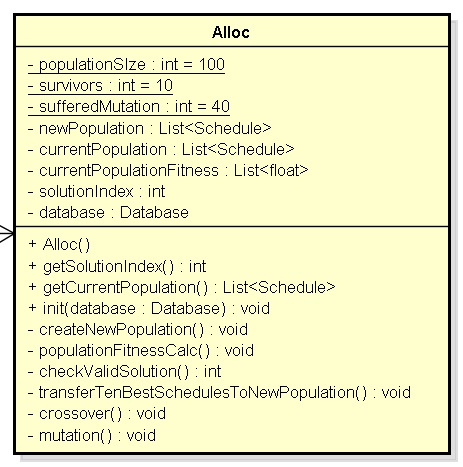
\includegraphics[width=0.6\textwidth]{Alloc.jpg}
\caption{\label{fig:alloc}Class Alloc}
\end{figure}


\subsection{Class Building}
\begin{figure}[H]
\centering
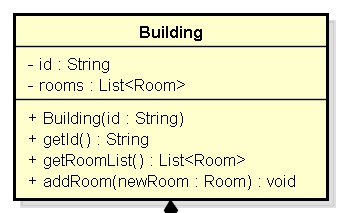
\includegraphics[width=0.4\textwidth]{Building.jpg}
\caption{\label{fig:building}Class Building}
\end{figure}


\subsection{Class Course}
\begin{figure}[H]
\centering
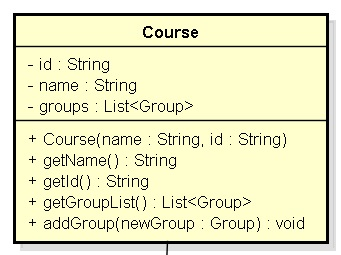
\includegraphics[width=0.4\textwidth]{Course.jpg}
\caption{\label{fig:course}Class Course}
\end{figure}


\subsection{Class Database}
\begin{figure}[H]
\centering
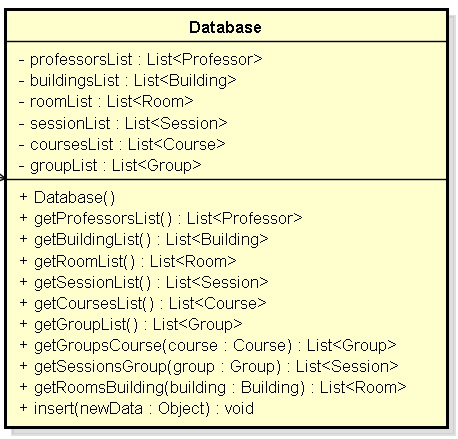
\includegraphics[width=0.6\textwidth]{Database.jpg}
\caption{\label{fig:database}Class Database}
\end{figure}


\subsection{Class Group}
\begin{figure}[H]
\centering
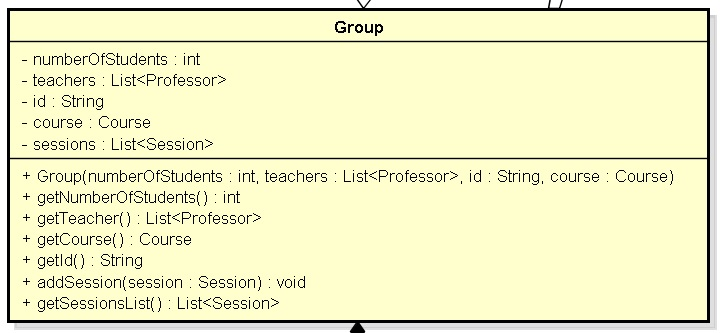
\includegraphics[width=0.8\textwidth]{Group.jpg}
\caption{\label{fig:group}Class Group}
\end{figure}


\subsection{Class INFOperationService - Interface}
\begin{figure}[H]
\centering
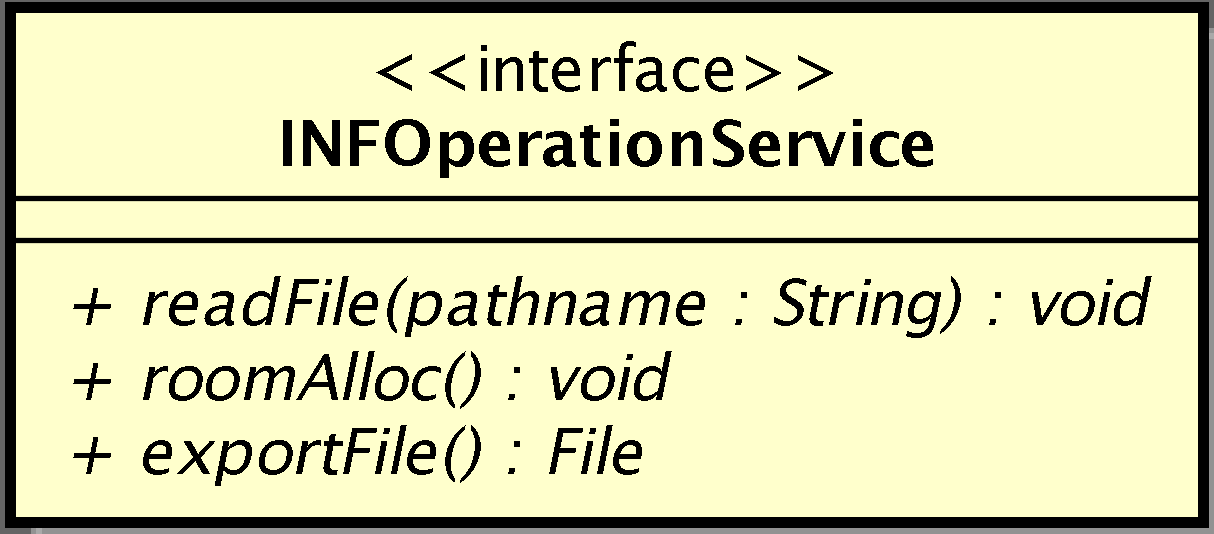
\includegraphics[width=0.4\textwidth]{OpServ.png}
\caption{\label{fig:OpServ}Class INFOperationService <<interface>>}
\end{figure}


\subsection{Class INFOperationServiceImplementation}
\begin{figure}[H]
\centering
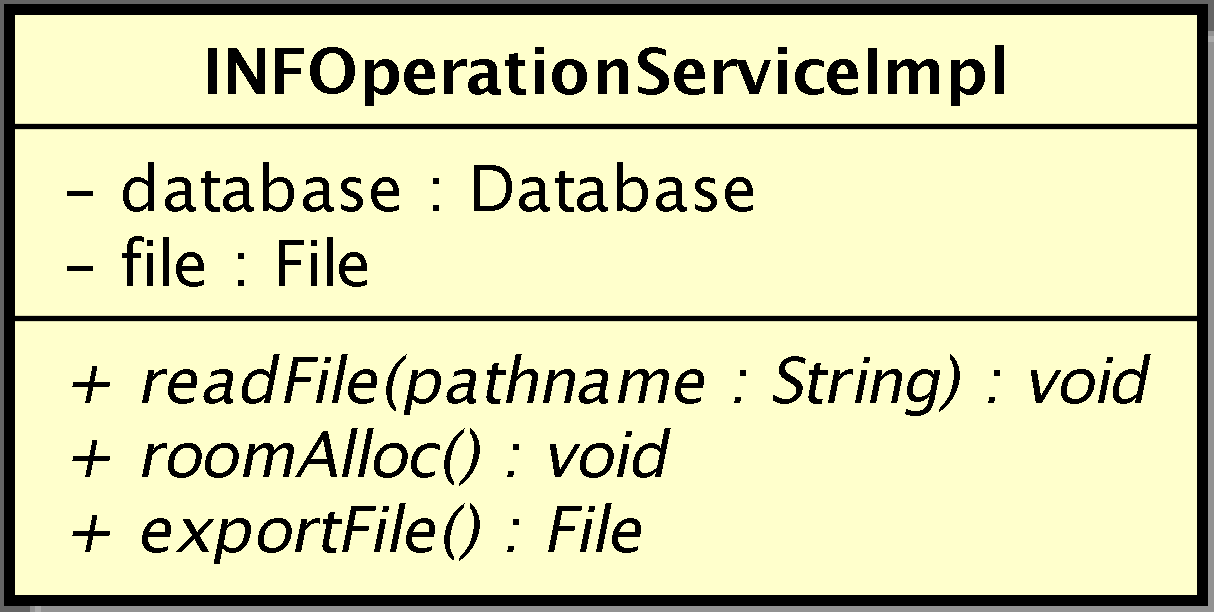
\includegraphics[width=0.4\textwidth]{OpServImpl.png}
\caption{\label{fig:OpServImpl}Class OpServImpl}
\end{figure}


\subsection{Class Professor}
\begin{figure}[H]
\centering
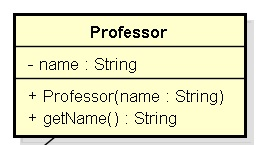
\includegraphics[width=0.4\textwidth]{Professor.jpg}
\caption{\label{fig:Professor}Class Professor}
\end{figure}


\subsection{Class Room}
\begin{figure}[H]
\centering
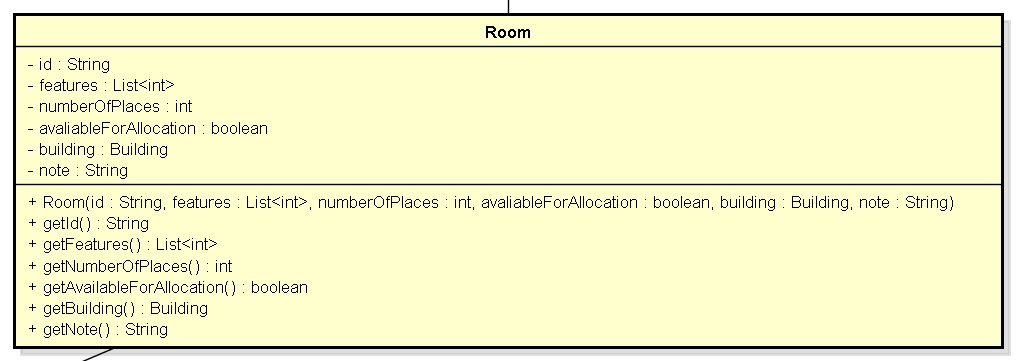
\includegraphics[width=0.8\textwidth]{Room.jpg}
\caption{\label{fig:room}Class Room}
\end{figure}


\subsection{Class Schedule}
\begin{figure}[H]
\centering
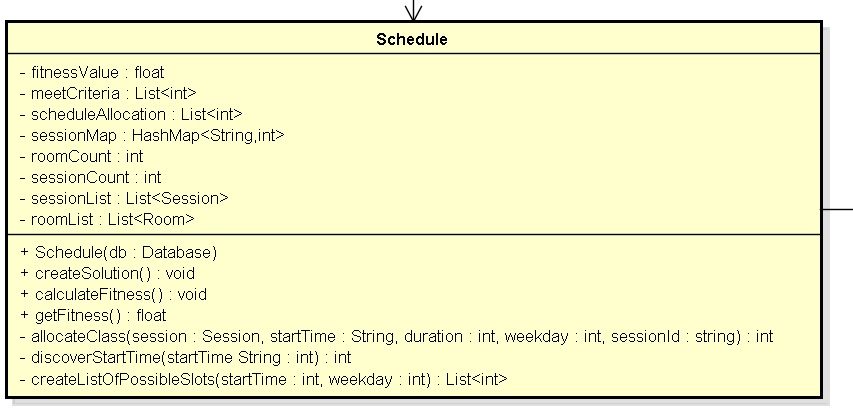
\includegraphics[width=0.8\textwidth]{Schedule.jpg}
\caption{\label{fig:schedule}Class Schedule}
\end{figure}


\subsection{Class Session}
\begin{figure}[H]
\centering
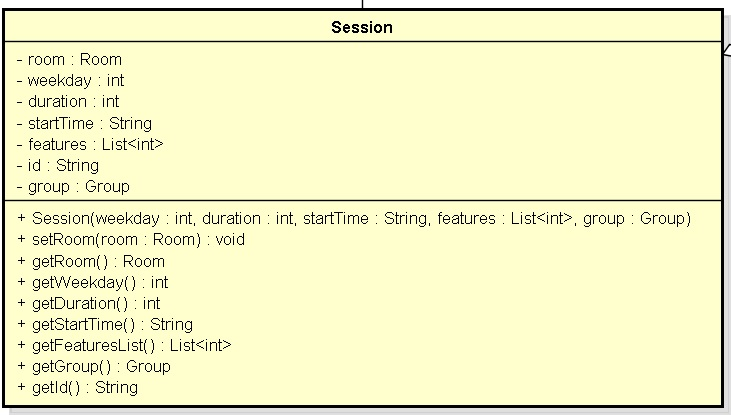
\includegraphics[width=0.8\textwidth]{session.jpg}
\caption{\label{fig:session}Class Session}
\end{figure}


\subsection{Class InputFile}
\begin{figure}[H]
\centering
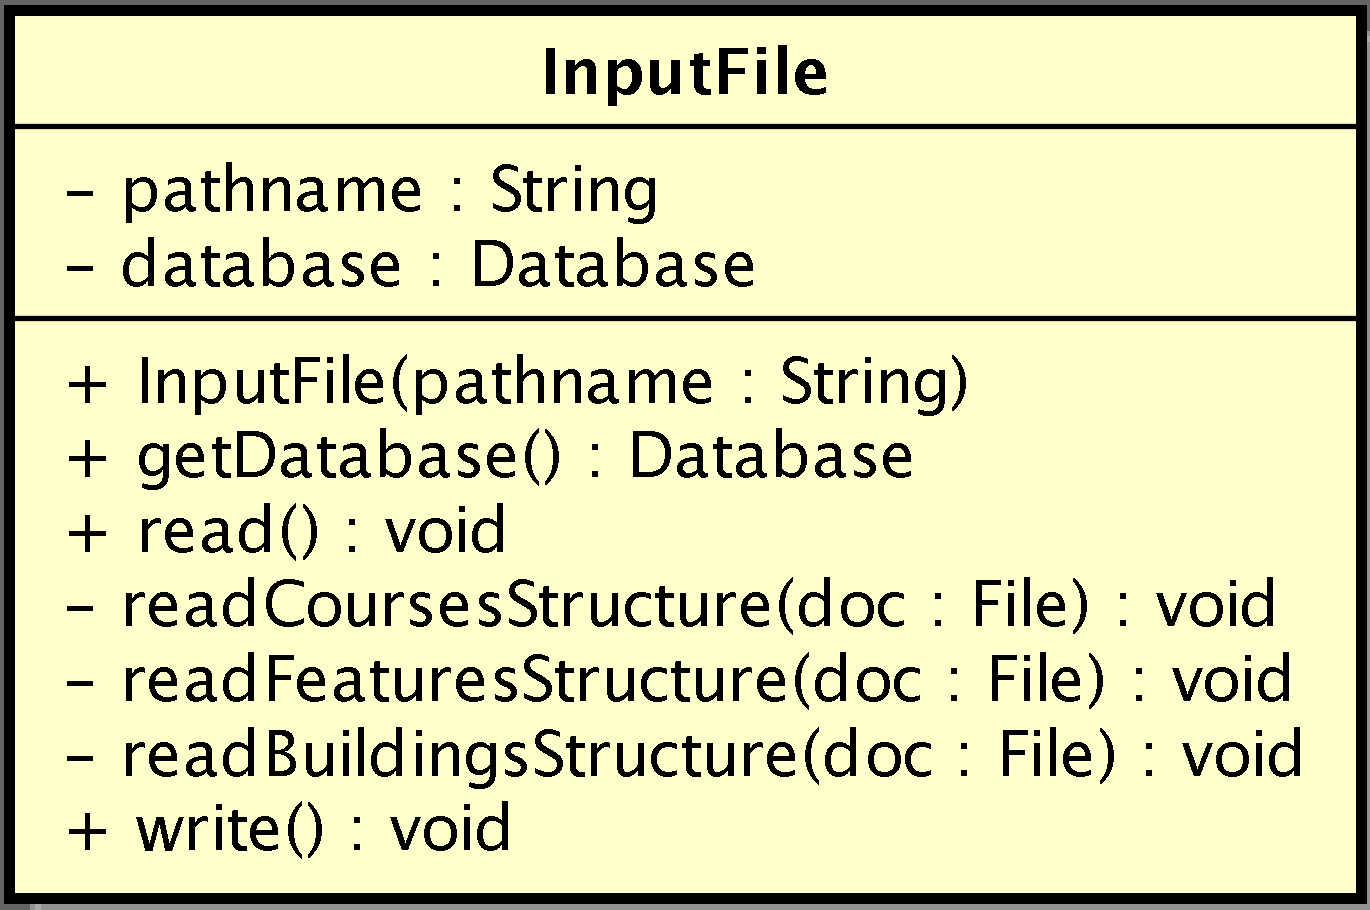
\includegraphics[width=0.4\textwidth]{InputFile.png}
\caption{\label{fig:InputFile}Class InputFile}
\end{figure}

\section{Relacionamentos}
\subsection{Architecture model}
\begin{figure}[H]
\centering
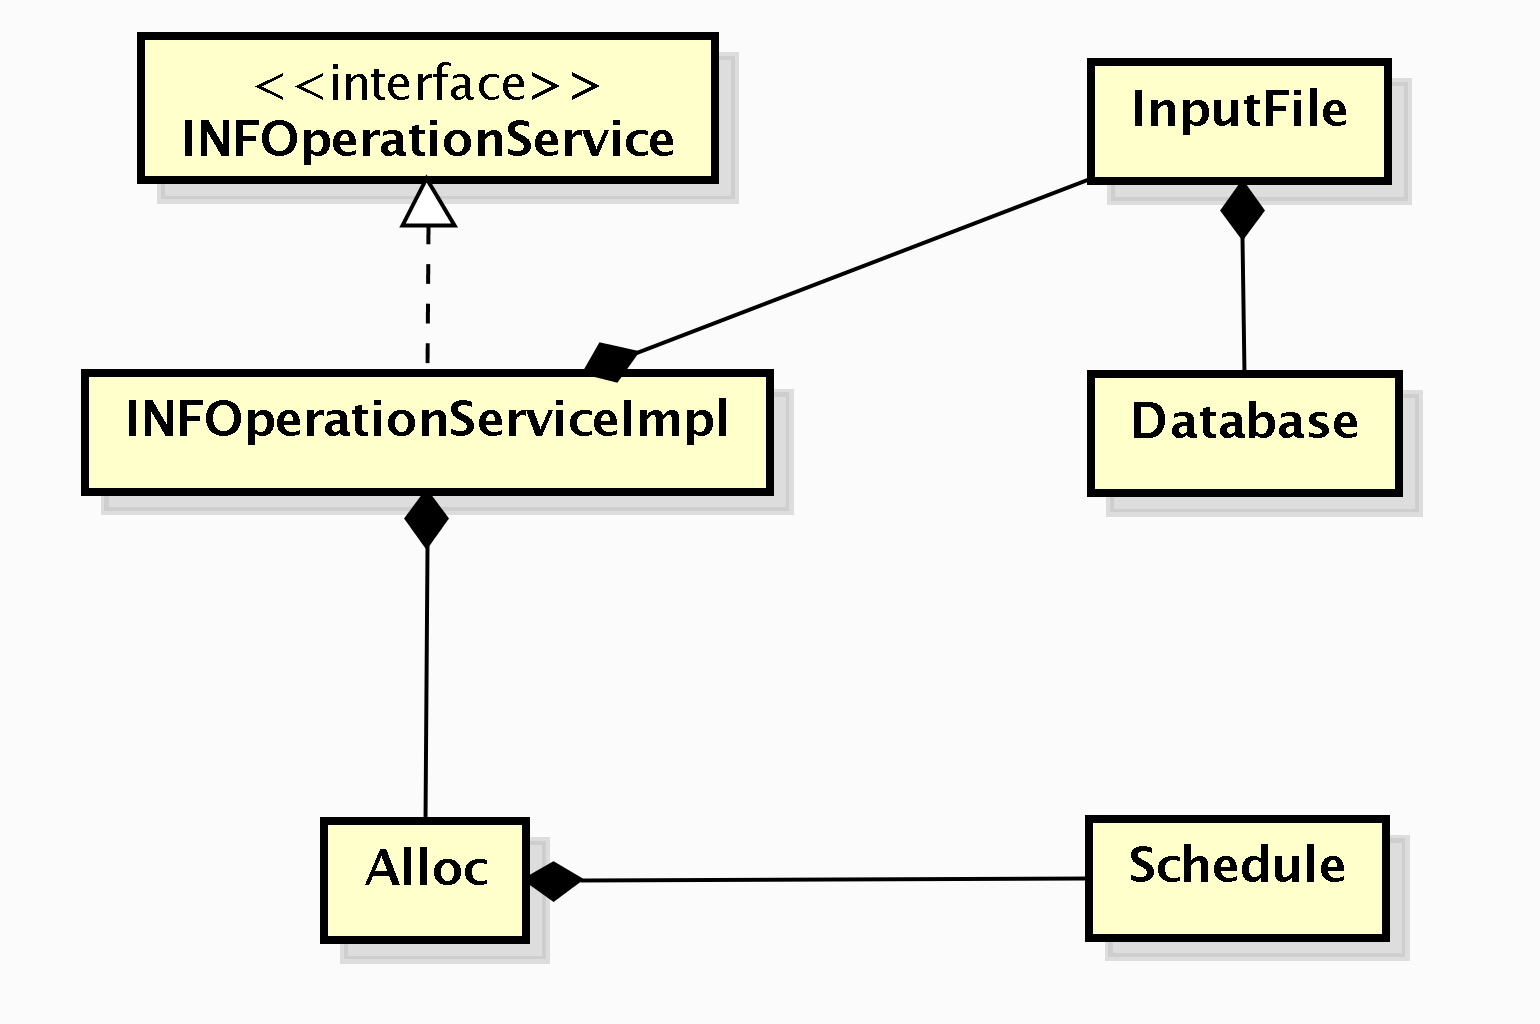
\includegraphics[width=0.6\textwidth]{ArchictectureModel.png}
\caption{\label{fig:ArchitectureModel}Relacionamentos entre as classes do Architecture Model}
\end{figure}

\subsection{Domain model}
\begin{figure}[H]
\centering
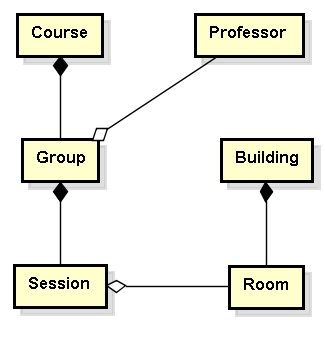
\includegraphics[width=0.4\textwidth]{domainModel.jpg}
\caption{\label{fig:domainModel}Relacionamentos entre as classes do Domain Model}
\end{figure}

\section{Critérios de qualidade}

\subsection{Qualidade interna}
\subsubsection{Modularidade}
Utilizar os critérios de modularidade visando garantir a maior independência possível entre as funções, possibilitando futuras alterações específicas que não alteram o comportamento do sistema como um todo. \\\
As classes e os métodos a elas relacionados terão papéis específicos no sistema, com "baixa responsabilidade", evitando que uma única classe ou um único método tenham influência sobre uma grande área do sistema.

\subsubsection{Legibilidade}
Essencial para a manutenção e compreensão do código, a legibilidade é alcançada definindo-se alguns critérios de escrita para o código.

\begin{itemize}
\item Idioma:  o código foi escrito em \textbf{inglês}.
\item  Nomenclatura:
\par \underline{Classes:} primeira letra de cada palavra em caixa alta.
\par \textit{Ex.: MyClass \\\ MyClass() <<construtor>> \\\ OBS.: construtores, ainda que sejam métodos, precisam ter o mesmo nome da classe para funcionar.}
\par \underline{Variáveis, atributos e métodos:}  primeira letra minúscula e caixa alta para cada palavra nova.
\par \textit{Ex.: myAttribute \\\ getAttribute()}

\par \underline{Documentação:}  o código foi escrito de modo a ser o mais auto-explicativo possível, trazendo mais liberdade em relação a comentários (que tendem a ficar obsoletos).\\\ Nesse aspecto, os critérios de nomenclatura citados acima são estendidos, uma vez que além da disposição das letras em caixa alta, o nome de cada classe/método/atributo foi explícito em relação ao papel de tal entidade.

\par \underline{Manutenabilidade:} Criamos funções compreensíveis e independentes de modo que sua manutenção tenha custo e tempo reduzido.

\par \underline{Funcionabilidade:} Visamos a entrega de um programa que executa os requisitos de forma precisa, atendendo às especificações do trabalho.

\par \underline{Confiabilidade:}
Além da entrega conforme as especificações do trabalho, visamos também informar o usuário de falhas como entrada não suportada, solução impossível e erros em geral.
\end{itemize}

\subsection{Qualidade externa}
A partir dos critérios de qualidade interna acima definidos, buscamos trazer para nosso sistema alguns critérios de qualidade visíveis ao usuário, ou seja, de qualidade externa. \\\
São eles: \textbf{robustez}, \textbf{corretude}, \textbf{compatibilidade} e \textbf{facilidade de uso}.
O usuário poderá usar facilmente um sistema que responderá bem a situações adversas às que foram programadas, assim como atenderá bem às tarefas especificadas.


\end{document}
